\documentclass[UTF8,a4paper,11pt,fontset=fandol]{ctexart}
\usepackage[margin=2.2cm]{geometry}
\usepackage{amsmath,amssymb,booktabs}
\usepackage{graphicx}
\setlength{\parskip}{0.3em}
\linespread{1.1}

\begin{document}
\pagestyle{plain}

\begin{center}
  {\Large\bfseries 例2.3：热扩散问题}
\end{center}

\section{原题抄录}

考虑图2.4(a)中由 $100\times100$ 个节点组成的网络，其中每个节点都和其
上下左右的节点相邻（由于节点的密度原因没有显式标出来）。假设(a)图内部
阴影区域的节点处在热源，使得它们的温度固定在 $1$（这里温度就当作势能
考虑）。图中最上面一层和最下面一层的节点被假设为绝热使得它们的温度在
$0$，而其他节点不受到激励者放散热。通过求解方程(2.36)（需要对
$100\times100$ 的节点进行向量化，并且假设式(2.37)中 $r=1$），可以得到
所有节点的温度分布，如图2.4(b)所示。


\section{代码的结构、算法说明}

程序首先设置网格规模。令每一维包含 $n=100$ 个节点，则总节点数为
\[
N=n^2=10000.
\]
由于 $100\times100$ 的规则网格中水平方向共有
$100\times99$ 条边，竖直方向同样共有 $99\times100$ 条边，因此网格中的
总边数为
\[
m=2n(n-1)=19800.
\]

程序使用二维布尔数组 \texttt{heat} 表示热源所在位置。首先将数组初始化为
全 \texttt{False}，再根据题目图2.4(a)中三个阴影区域将相应节点设置为
\texttt{True}：
\[
\texttt{heat[19:23,67:90]}=\texttt{True},
\]
\[
\texttt{heat[67:87,18:22]}=\texttt{True}.
\]
此外，通过循环
\[
\texttt{heat[i-1,i-1:i+5]=True},
\qquad i=40,\ldots,67,
\]
构造图中的斜向热源区域。这里数组下标从 $0$ 开始，因此程序中的数组下标
比图中的行、列编号小 $1$。

随后令
\[
\texttt{fixed}=\texttt{heat.copy()},
\]
将所有热源节点设置为固定温度节点，并通过
\[
\texttt{fixed[[0,-1],:]=True}
\]
将最上面和最下面两行节点也设置为固定节点。因此，\texttt{fixed} 用于记录
哪些节点的温度已经给定。


\subsection*{（1）关联矩阵 $A$ 的构造}

程序没有直接构造离散拉普拉斯矩阵 $L$，而是按照教材中的方法首先构造
节点--边关联矩阵 $A$，然后计算
\[
\boxed{L=AA^{\mathrm T}}.
\]

将二维网格中的节点按照从上到下、从左到右的顺序编号。对于坐标为
$(i,j)$ 的节点，其一维编号为
\[
\boxed{k=in+j}.
\]
因此二维的 $100\times100$ 个节点被转换成一个长度为 $10000$ 的一维节点
向量。

关联矩阵 $A$ 的每一列对应网格中的一条边。对于一条连接节点 $p$ 和 $q$
的边，规定在对应列中
\[
A_{p,e}=1,\qquad A_{q,e}=-1,
\]
其余元素均为 $0$。因此，每一列恰好只有两个非零元素。

程序使用
\texttt{edge} 表示当前边的编号。边的编号按照节点从上到下、从左到右
的顺序进行，并且对于每一个节点，先处理与右侧节点的连接，再处理与下方
节点的连接。

当当前节点为 $k$ 时，如果它存在右侧邻点，则右侧节点编号为
\[
q=k+1.
\]
程序执行
\[
A_{k,e}=1,\qquad A_{k+1,e}=-1,
\]
然后令
\[
e\leftarrow e+1.
\]

如果当前节点存在下方邻点，则下方节点编号为
\[
q=k+n.
\]
程序执行
\[
A_{k,e}=1,\qquad A_{k+n,e}=-1,
\]
然后令
\[
e\leftarrow e+1.
\]

由于边的编号本质上只是对矩阵 $A$ 的列进行编号，因此只要每条边都被
正确表示，改变边的编号顺序并不会影响最终的 $L$。例如若通过列置换矩阵
$P$ 改变边的编号，则
\[
A'=AP,
\]
从而
\[
A'A'^{\mathrm T}
=APP^{\mathrm T}A^{\mathrm T}
=AA^{\mathrm T}.
\]

最终得到
\[
A\in\mathbb{R}^{10000\times19800}.
\]


\subsection*{（2）由 $A$ 得到离散拉普拉斯矩阵 $L$}

程序通过

\[
\texttt{L=A@A.T}
\]

计算
\[
\boxed{L=AA^{\mathrm T}}.
\]

对于任意节点 $i$，矩阵 $L$ 的对角元素为该节点与其他节点相连的边数，即
\[
L_{ii}=\deg(i).
\]
如果两个不同节点 $i,j$ 之间存在一条边，则
\[
L_{ij}=L_{ji}=-1;
\]
如果两个节点之间不存在直接连接关系，则
\[
L_{ij}=0.
\]

因此，
\[
L_{ij}=
\begin{cases}
\deg(i),&i=j,\\
-1,&i\ne j\text{ 且 }i,j\text{ 相邻},\\
0,&\text{其他情况}.
\end{cases}
\]

由此得到一个 $10000\times10000$ 的稀疏矩阵 $L$。

采用稀疏矩阵存储的原因是虽然矩阵 $L$ 的规模达到
$10000\times10000$，但每一个节点只与有限个邻点相连，因此每一行只有
少量非零元素。使用稀疏矩阵可以显著降低存储和计算所需的资源。


\subsection*{（3）固定节点与非固定节点}

程序定义
\[
I=\texttt{eye}(N),
\]
即 $10000\times10000$ 的单位矩阵。

根据 \texttt{fixed} 数组构造对角矩阵
\[
C=\operatorname{diag}(\texttt{fixed}),
\]
其中固定温度节点对应的对角元素为 $1$，非固定节点对应的对角元素为
$0$。

再定义
\[
B=I-C.
\]

因此对于固定节点，
\[
C_{ii}=1,\qquad B_{ii}=0,
\]
而对于非固定节点，
\[
C_{ii}=0,\qquad B_{ii}=1.
\]

于是
\[
\boxed{B+C=I}.
\]

同时，将二维热源数组展平成长度为 $10000$ 的向量
\[
d=\texttt{heat.ravel().astype(float)}.
\]
因此热源节点对应的 $d_i=1$，其他节点对应的 $d_i=0$。


\subsection*{（4）分块线性方程组}

程序最终构造分块矩阵
\[
M=
\begin{pmatrix}
I&-L\\
B&C
\end{pmatrix},
\]
并求解
\[
\boxed{
\begin{pmatrix}
I&-L\\
B&C
\end{pmatrix}
\begin{pmatrix}
s\\
e
\end{pmatrix}
=
\begin{pmatrix}
0\\
d
\end{pmatrix}.
}
\]

将其展开，可以得到
\[
\begin{cases}
s-Le=0,\\
Bs+Ce=d.
\end{cases}
\]

由第一式得到
\[
s=Le.
\]
代入第二式可得
\[
BLe+Ce=d,
\]
即
\[
\boxed{(BL+C)e=d}.
\]

这个方程同时描述了固定节点和非固定节点的条件。

对于非固定节点，有
\[
B_{ii}=1,\qquad C_{ii}=0,
\]
因此对应方程为
\[
(Le)_i=d_i.
\]
由于非固定节点不是热源，所以 $d_i=0$，从而
\[
\boxed{(Le)_i=0}.
\]

这正是稳态热扩散问题的离散拉普拉斯方程，即内部节点的温度满足与
相邻节点之间的平衡关系。

对于固定温度节点，有
\[
B_{ii}=0,\qquad C_{ii}=1,
\]
因此对应方程为
\[
e_i=d_i.
\]
对于热源节点，$d_i=1$，所以
\[
\boxed{e_i=1}.
\]
而最上面和最下面两行虽然也是固定节点，但不属于热源，因此
\[
d_i=0,
\]
从而
\[
\boxed{e_i=0}.
\]

因此，该分块方程组将热扩散方程和固定温度条件统一到一个线性方程组
中进行求解。

程序最后使用
\texttt{spsolve(M,rhs)} 对这个稀疏线性方程组进行求解，并将得到的
$20000$ 维解向量分成两个长度为 $10000$ 的向量 $s$ 和 $e$，其中
$e$ 即所有网格节点的温度。


\section{输出结果呈现}

运行最终代码后得到所有节点的温度分布。程序通过

\[
\texttt{e.reshape(n,n)}
\]

将长度为 $10000$ 的温度向量重新恢复为 $100\times100$ 的二维矩阵，
并利用 \texttt{imshow} 绘制温度分布图。

图中采用灰度色图，并设置
\[
0\leq e_{i,j}\leq1.
\]
颜色越接近黑色表示温度越接近 $0$，颜色越接近白色表示温度越接近
$1$。

\begin{center}
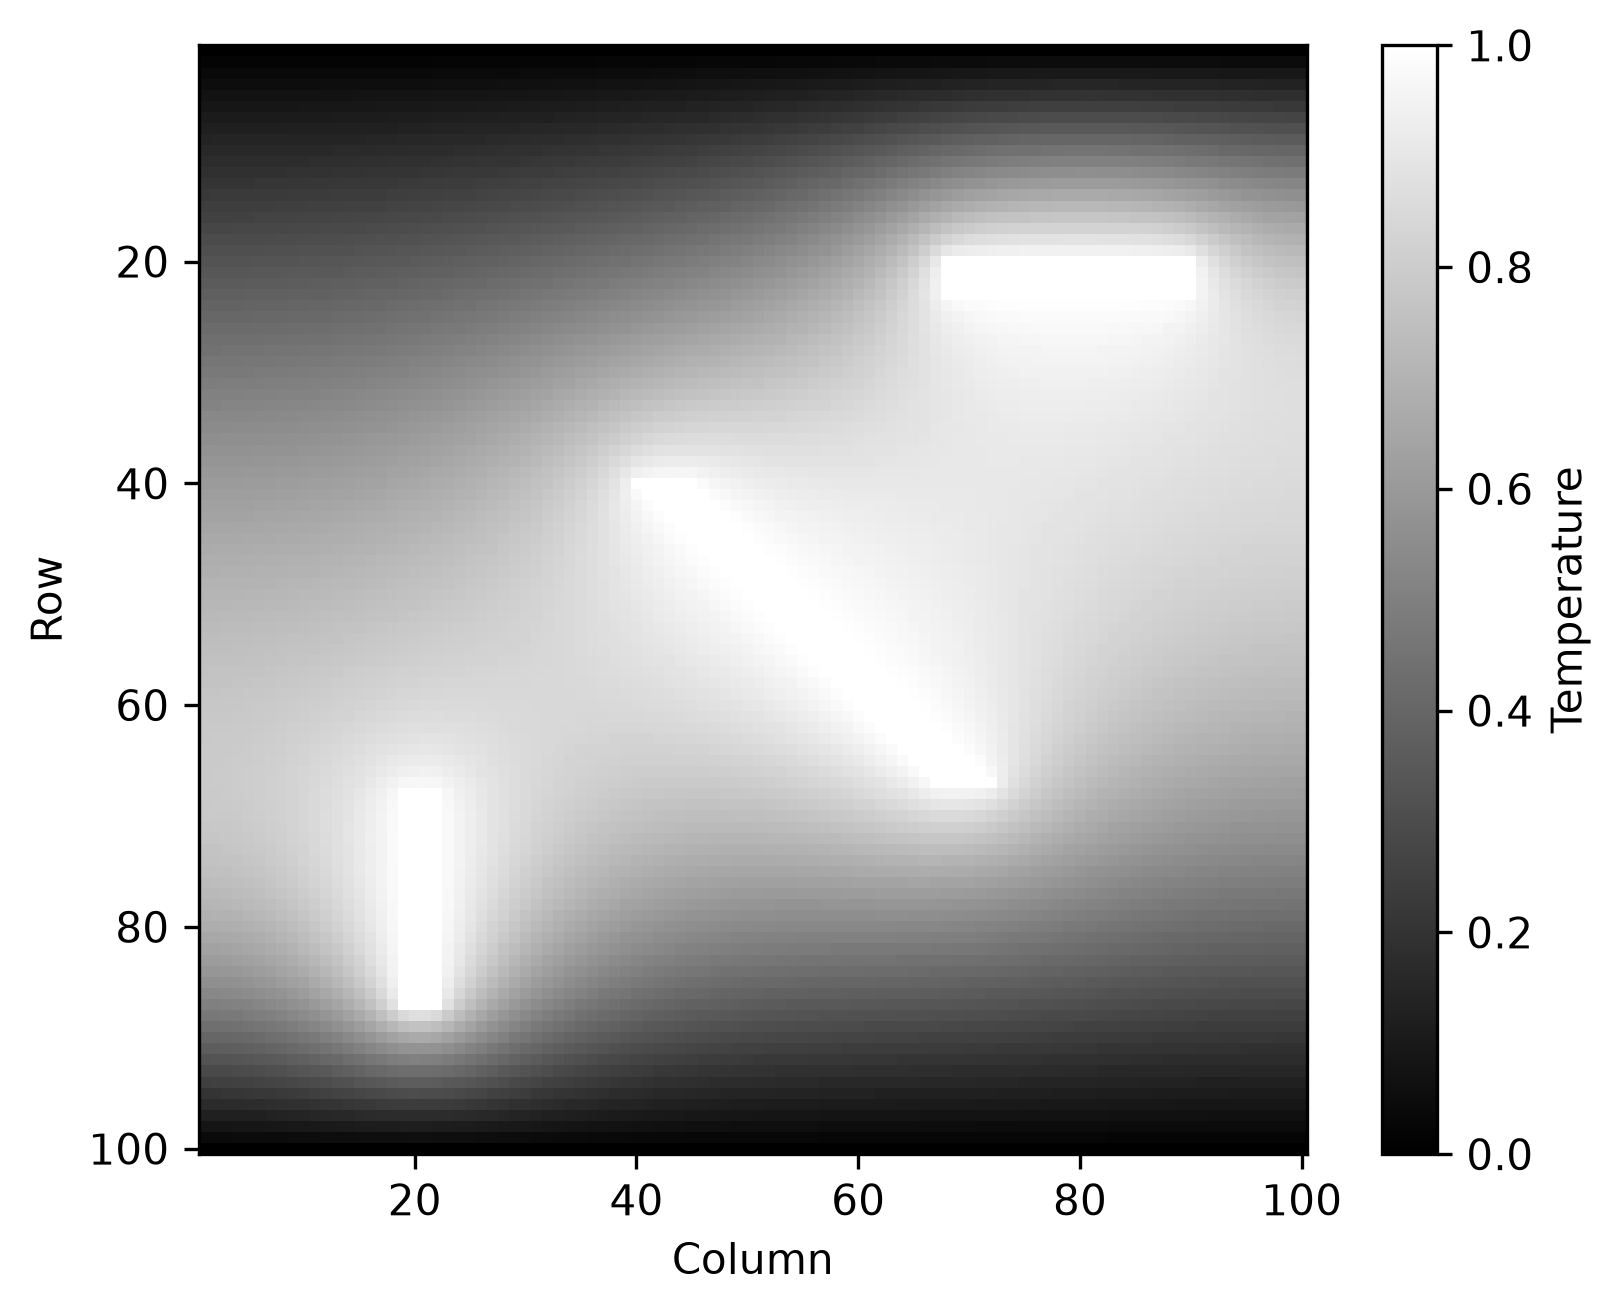
\includegraphics[width=0.78\textwidth]{heat_diffusion.png}
\end{center}

\begin{center}
图1\quad $100\times100$ 网格上的稳态温度分布
\end{center}

程序计算得到的解满足
\[
\min_i e_i=0,
\]
而最大温度为
\[
\max_i e_i\approx1.0000000000000013.
\]

由于浮点数计算存在舍入误差，理论上的最大值 $1$ 在程序中可能表现为
略大于 $1$ 的数值，但其误差处于浮点计算精度范围内。

此外，对最终分块方程组的残差进行检验：
\[
r=
M
\begin{pmatrix}
s\\e
\end{pmatrix}
-
\begin{pmatrix}
0\\d
\end{pmatrix}.
\]
程序计算得到
\[
\boxed{
\|r\|_\infty
\approx4.11\times10^{-15}.
}
\]

因此数值解能够非常准确地满足所构造的分块线性方程组。


\section{对输出结果的分析和结论}

本实验将 $100\times100$ 的二维热扩散问题离散为包含 $10000$ 个节点的
网络。首先按照节点之间的相邻关系构造节点--边关联矩阵 $A$，其中
每条边对应 $A$ 的一列，并在两个端点位置分别取 $1$ 和 $-1$。由此得到
\[
A\in\mathbb{R}^{10000\times19800}.
\]

进一步通过
\[
L=AA^{\mathrm T}
\]
得到网络的离散拉普拉斯矩阵。矩阵 $L$ 的对角元素表示节点的邻点数，
非对角元素在相邻节点之间取 $-1$，从而完整描述了网格中各节点之间的
传递关系。

在此基础上，程序利用矩阵 $B$ 和 $C$ 区分固定温度节点和非固定温度
节点，并通过
\[
\begin{pmatrix}
I&-L\\
B&C
\end{pmatrix}
\begin{pmatrix}
s\\e
\end{pmatrix}
=
\begin{pmatrix}
0\\d
\end{pmatrix}
\]
统一表示稳态热扩散方程和边界条件。消去辅助变量 $s$ 后，可以得到
\[
(BL+C)e=d.
\]
因此，对于非固定节点，该方程要求离散拉普拉斯为零；对于固定节点，
则直接规定节点温度，从而实现了题目所要求的热源和边界条件。

从最终温度分布图可以看到，热源区域的温度保持在 $1$，最上面和最下面
两行节点的温度保持在 $0$。热量从内部的高温热源区域向周围节点扩散，
在非固定节点处逐渐形成平滑的温度变化。由于左右边界没有被设置为固定
温度节点，热量在这些方向上的传播由网格内部的连接关系自然确定。

最终计算得到的分块线性方程组无穷范数残差约为
\[
4.11\times10^{-15},
\]
说明稀疏线性方程组求解器得到的数值解具有较高的计算精度。

综上，本实验通过构造关联矩阵 $A$ 并计算
\[
L=AA^{\mathrm T},
\]
成功将二维热扩散问题转化为大规模稀疏线性方程组，并利用稀疏矩阵方法
得到所有节点的稳态温度分布。计算结果符合热扩散问题的物理规律，并且
残差处于机器浮点精度范围内，验证了所构造模型和数值求解方法的正确性。

\end{document}